\documentclass[12pt, a4paper]{article}

% Preamble
% Paquetes para idioma, gráficos, matemáticas y formato.
\usepackage[spanish]{babel}
\usepackage[utf8]{inputenc}
\usepackage{graphicx}
\usepackage{amsmath}
\usepackage{geometry}
\usepackage{titlesec}
\usepackage{wrapfig}
\usepackage{hyperref}

% Configuración del documento
\titlespacing*{\section}{0pt}{1.5\baselineskip}{1.5\baselineskip}
\newcommand{\sectionbreak}{\clearpage}
\geometry{a4paper, left=2.5cm, right=2.5cm, top=2.5cm, bottom=2.5cm}
\title{Propuesta de Trabajo de Fin de Grado - Integración de Metrología y Robótica Colaborativa para la Inspección de Piezas en un Entorno Industrial Flexible}
\author{Alexander Kalis} 
\date{\today}

% Inicio del documento
\begin{document}

\maketitle
\thispagestyle{empty}
\newpage 

\begin{abstract}
La presente propuesta de Trabajo de Fin de Grado (TFG) describe el diseño y la implementación de una celda de manufactura flexible y automatizada,
orientada a la inspección de piezas mediante metrología. El proyecto integra un robot colaborativo Dobot CR5 con un sistema de visión 
3D para la tarea de bin-picking, el cual selecciona piezas de forma aleatoria de un contenedor. Estas piezas son posteriormente
transferidas a una máquina de metrología Zeiss DuraMax, que verifica su calidad. La gestión y el control de los procesos se llevan
a cabo a través de un controlador lógico programable (PLC) Siemens, que orquesta la comunicación entre los diferentes dispositivos. 
Este sistema, concebido como una instalación de demostración para la feria industrial Bienal Internacional de Máquina-Herramienta (BIEMH) de Bilbao (Q1 2026), tiene como objetivo principal 
mostrar la viabilidad y las ventajas de la integración de tecnologías de robótica, visión artificial y metrología en un entorno de
producción real, optimizando la precisión y la eficiencia en la cadena de valor de la industria 4.0.
\end{abstract}

\newpage
\tableofcontents
\newpage
\section{Introducción}
El sector industrial se encuentra en una fase de profunda transformación, impulsada por los principios de la Industria 4.0, que abogan por una integración total de la tecnología digital en los procesos de fabricación. Esta evolución exige sistemas de producción más inteligentes y flexibles, capaces de adaptarse a la demanda de alta precisión y control de calidad en tiempo real. En este contexto, la robótica colaborativa y los sistemas de visión artificial emergen como pilares fundamentales para optimizar tareas complejas, como la manipulación de piezas en entornos desestructurados.

Con el objetivo de abordar estos desafíos, el presente proyecto se centra en el diseño y la implementación de una celda de manufactura automatizada. El sistema propuesto, que servirá como demostración en la prestigiosa feria industrial BIEMH en Bilbao, integra un robot colaborativo Dobot CR5 equipado con una garra Schunk y un sistema de visión 3D para la aplicación de \textit{bin-picking}. Este conjunto permite la selección autónoma de piezas de un contenedor de forma aleatoria, demostrando una capacidad de interacción con el entorno hasta ahora limitada a soluciones rígidas. Este proyecto es una propuesta personal que se enmarca en la actividad profesional que desarrollo en el centro de investigación aplicada Tekniker, lo que garantiza su aplicación en un entorno industrial real y de alta exigencia.

Una vez manipulada, la pieza es transferida a una máquina de metrología Zeiss DuraMax, donde se somete a una inspección de alta precisión que determina su conformidad. La coordinación de todos estos subsistemas de hardware, desde la robótica hasta la metrología, es orquestada por un PLC Siemens. Para ir más allá de la mera integración de componentes, como director del proyecto, supervisaré la implementación de un software adicional para el seguimiento de la producción. Este software de \textit{tracking} permitirá registrar datos clave sobre el rendimiento del sistema, la eficiencia del proceso y la calidad del producto, ofreciendo una visión completa de la operación desde una perspectiva de gestión y control de la producción. De esta forma, el proyecto no solo exhibe una solución tecnológica, sino que también establece las bases para una futura optimización de procesos a nivel de sistemas de información.

\section{Justificación y motivación}
Este proyecto de TFG se justifica por su relevancia en el marco de la transformación digital de la industria y su clara alineación con múltiples líneas de investigación propuestas por la comisión de TFG. La propuesta no solo aborda un problema de ingeniería real y de actualidad, sino que también integra una variedad de tecnologías avanzadas, demostrando un conocimiento transversal de la Ingeniería Industrial.

El proyecto se alinea con las siguientes líneas de investigación:

\subsection{Producción, planificación y control de la producción}
La inclusión de un software de \textit{tracking} de producción es fundamental en este punto. Este sistema permite monitorizar los indicadores clave de rendimiento (KPIs), como el número de piezas inspeccionadas y el tiempo de ciclo, estableciendo las bases para la optimización de la planificación y el control de los procesos de manufactura.

\subsection{Uso de herramientas informáticas aplicadas a la resolución de problemas de ingeniería}
La programación del robot colaborativo Dobot CR5, el desarrollo del sistema de visión 3D para \textit{bin-picking} y la integración de software de \textit{tracking} son ejemplos directos de cómo se aplican herramientas informáticas para resolver problemas complejos de automatización y producción. Adicionalmente, se generará una simulación con el software RoboDK previamente al montaje para asegurar que la celda es viable físicamente.

\subsection{Métodos cuantitativos, algoritmos, optimización, modelado y validación de sistemas industriales}
La implementación del algoritmo de \textit{bin-picking} para la selección de piezas de forma aleatoria es un claro ejemplo de la aplicación de algoritmos. El modelado y la simulación de la celda de trabajo son pasos clave en el diseño del proyecto para optimizar la eficiencia y la seguridad del sistema antes de su implementación física.

\subsection{Implementación de soluciones y tecnologías IT aplicadas a la ingeniería de organización industrial}
La integración de una red de comunicación entre el robot, la máquina de metrología, el PLC Siemens y el software de \textit{tracking} de producción representa la implementación de una solución tecnológica avanzada que mejora la gestión y la organización de los procesos industriales.

\subsection{Gestión para la organización y dirección de empresas, sistemas de información y gestión integrada (ERP)}
La función de director del proyecto y la implementación del software de \textit{tracking} van más allá de lo técnico, demostrando una comprensión de la gestión de proyectos y la importancia de los sistemas de información en el ámbito de la manufactura moderna.

\subsection{Gestión y supervisión de proyectos}
Como director de este proyecto, se aplicarán principios de gestión para asegurar el cumplimiento de objetivos y plazos, coordinando la integración de los distintos componentes y el desarrollo del software.

\subsection{Sistemas microcontrolados y sensorimetría aplicados a contexto industriales}
El uso del PLC Siemens para el control centralizado, así como la utilización de la cámara de visión 3D para la detección de piezas y la máquina de metrología Zeiss DuraMax para la sensórica de alta precisión, son elementos clave de esta línea.

En síntesis, este TFG demuestra una aplicación integral de conocimientos en áreas clave de la ingeniería, justificando su desarrollo y relevancia en el contexto de la industria actual.

\section{Descripción del proyecto}
El proyecto se centra en el diseño, implementación y validación de una celda de manufactura flexible y automatizada. La instalación integra una serie de componentes clave de hardware y software para llevar a cabo un ciclo de producción completo, desde la manipulación autónoma de piezas hasta su inspección de calidad.

\subsection{Arquitectura del sistema}
Como se puede ver en la Figura \ref{fig:arquitectura}, la celda de trabajo está diseñada bajo un enfoque modular, permitiendo la comunicación y la operación sincronizada de todos sus componentes. El PLC actúa como el cerebro del sistema, coordinando las secuencias de movimiento del robot, la comunicación con el sistema de visión 3D y la máquina de metrología. La red de comunicación asegura que el flujo de información sea bidireccional, permitiendo al PLC recibir datos de la cámara y de la máquina Zeiss DuraMax para tomar decisiones en tiempo real sobre la manipulación de las piezas y el control de calidad.

\begin{figure}[h!]
    \centering
    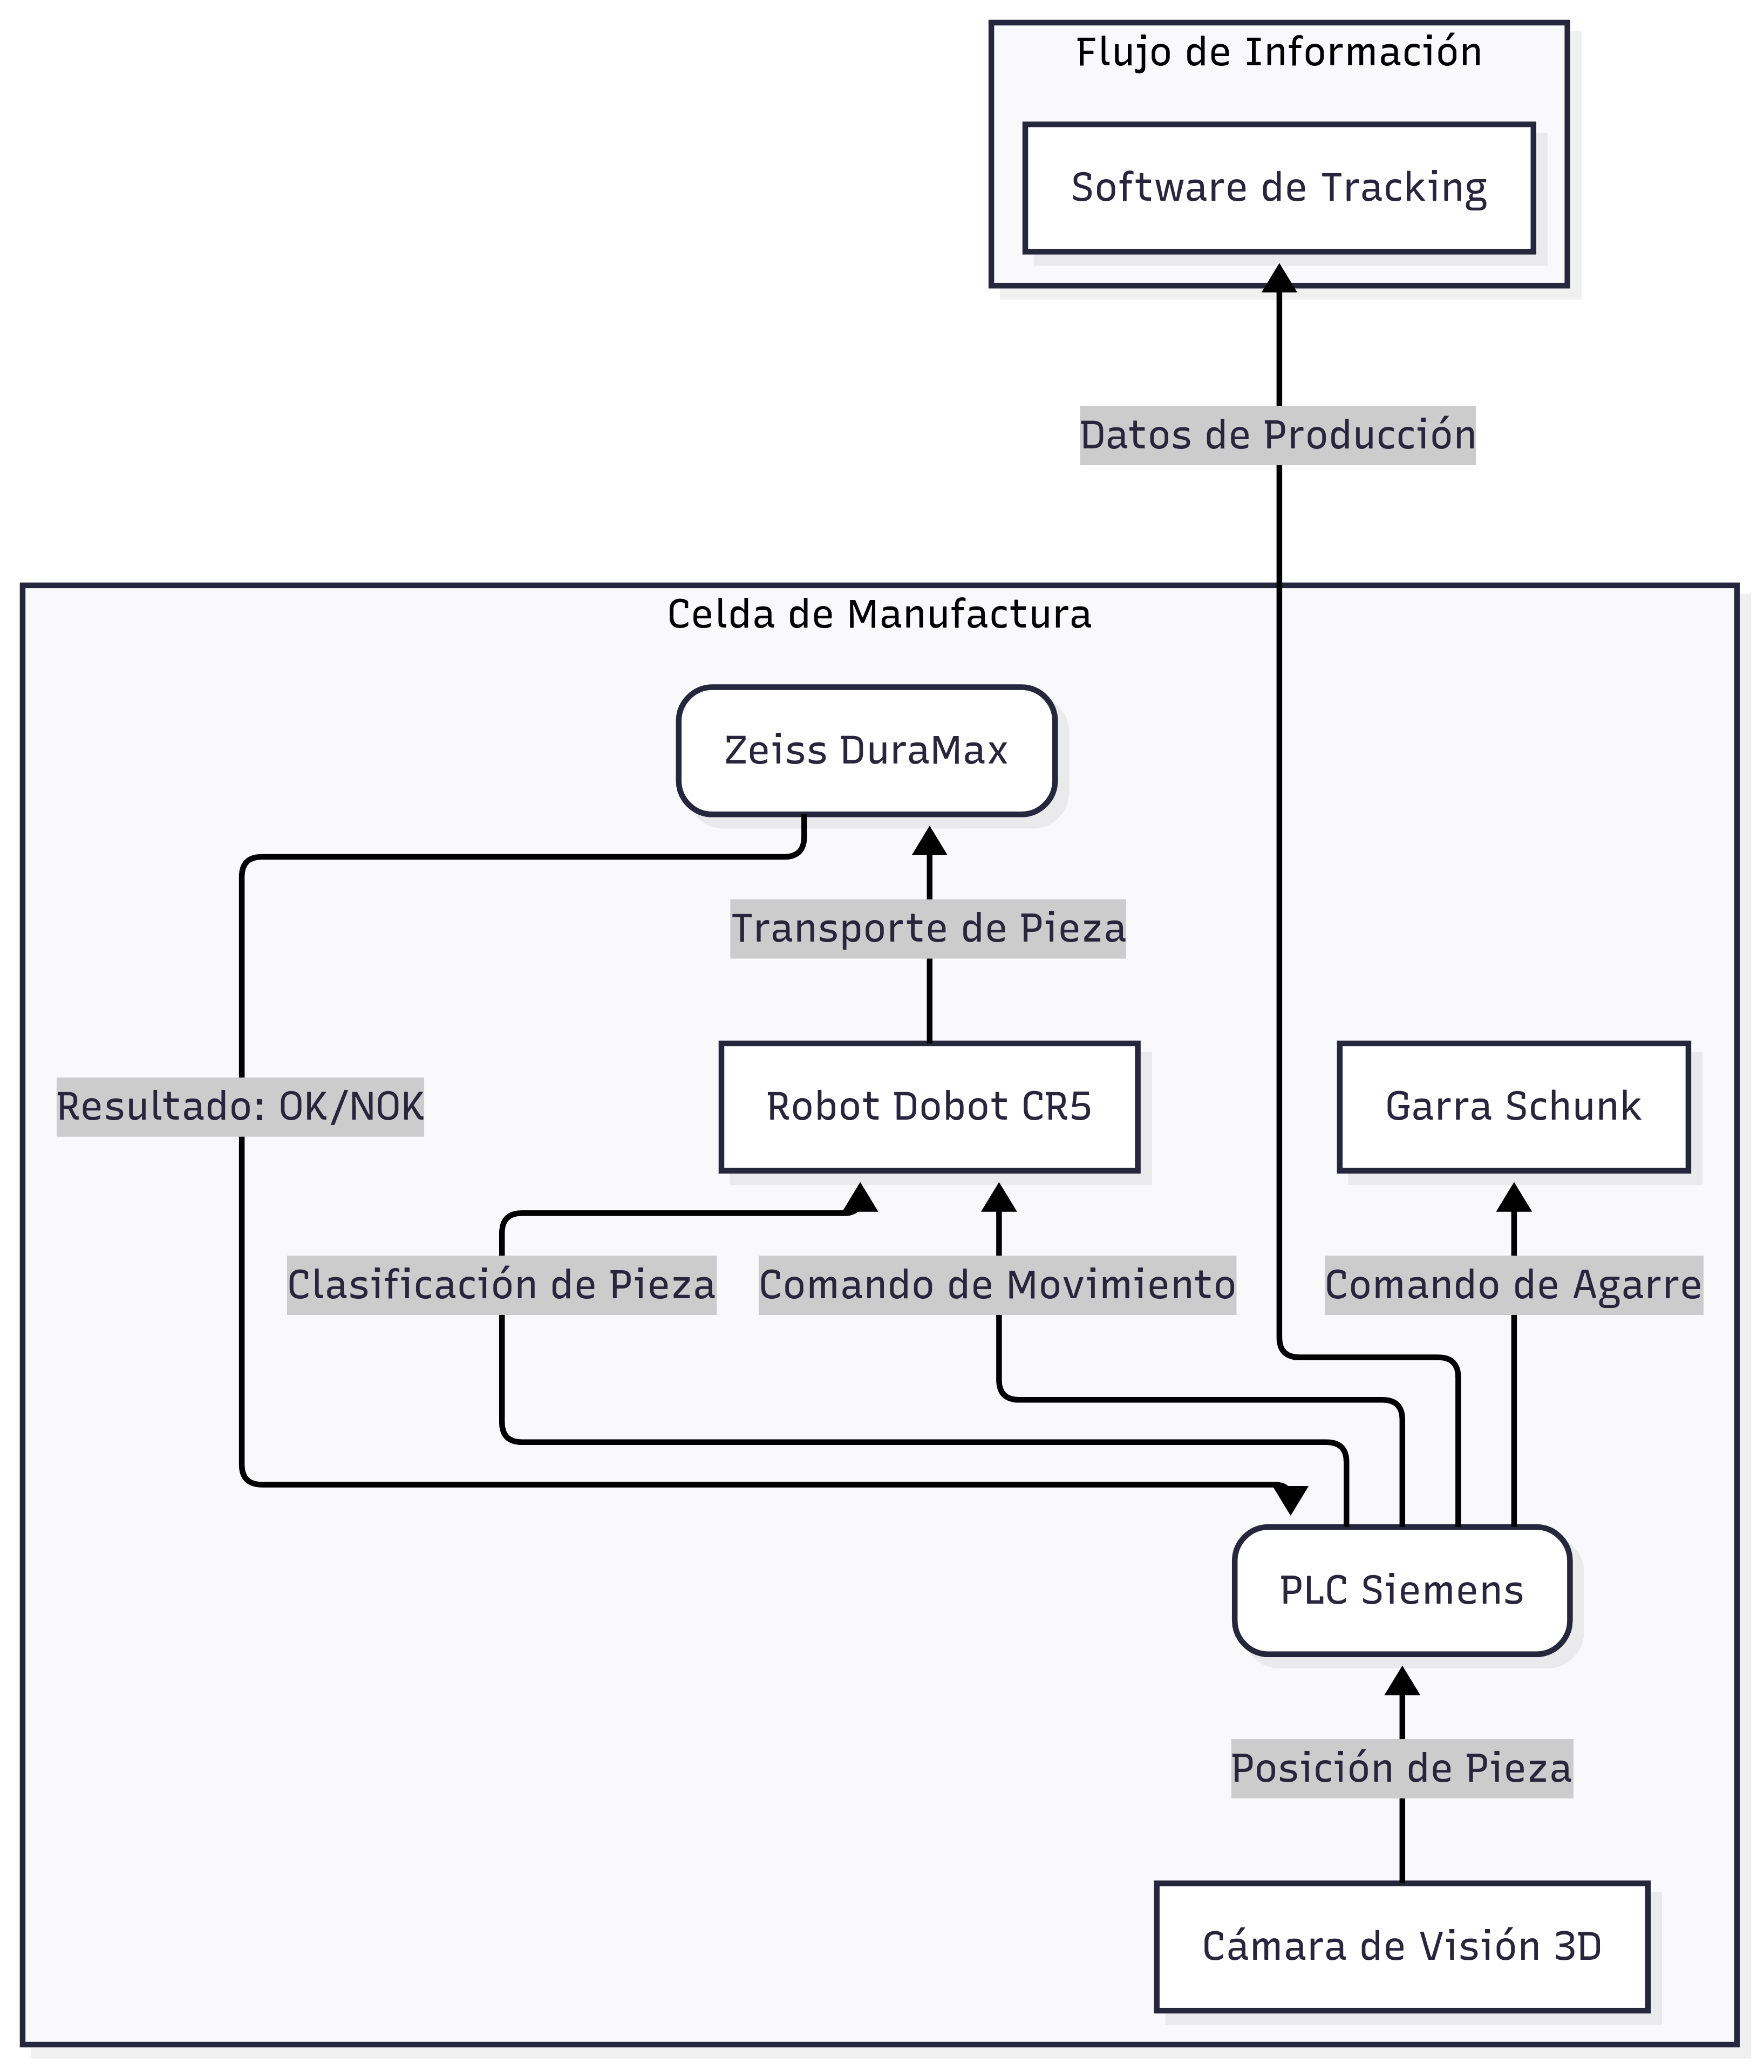
\includegraphics[width=0.75\textwidth]{arquitecturav2.png}
    \caption{Diagrama de arquitectura del sistema. Elaboración propia.}
    \label{fig:arquitectura}
\end{figure}

\subsection{Componentes clave}

\subsubsection{Robot colaborativo Dobot CR5}
Se utilizará el robot Dobot CR5 para la manipulación de piezas. Su naturaleza colaborativa permite una integración segura en un entorno de exposición como la BIEMH, eliminando la necesidad de vallas de seguridad y permitiendo la interacción con el público. La programación se centrará en el control de su cinemática para realizar tareas precisas de \textit{pick-and-place}.

\begin{figure}[h!]
    \centering
    \begin{minipage}{0.45\textwidth}
        \centering
        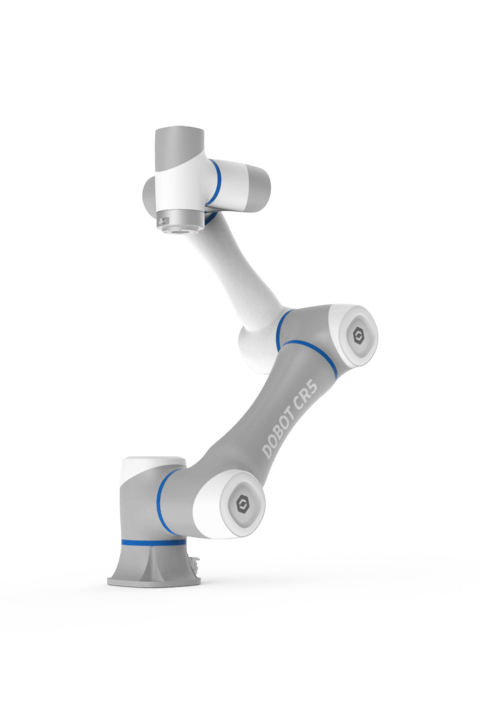
\includegraphics[width=\textwidth]{dobot.png}
        \caption{Dobot CR5}
        \label{fig:dobot}
    \end{minipage}\hfill
    \begin{minipage}{0.45\textwidth}
        \centering
        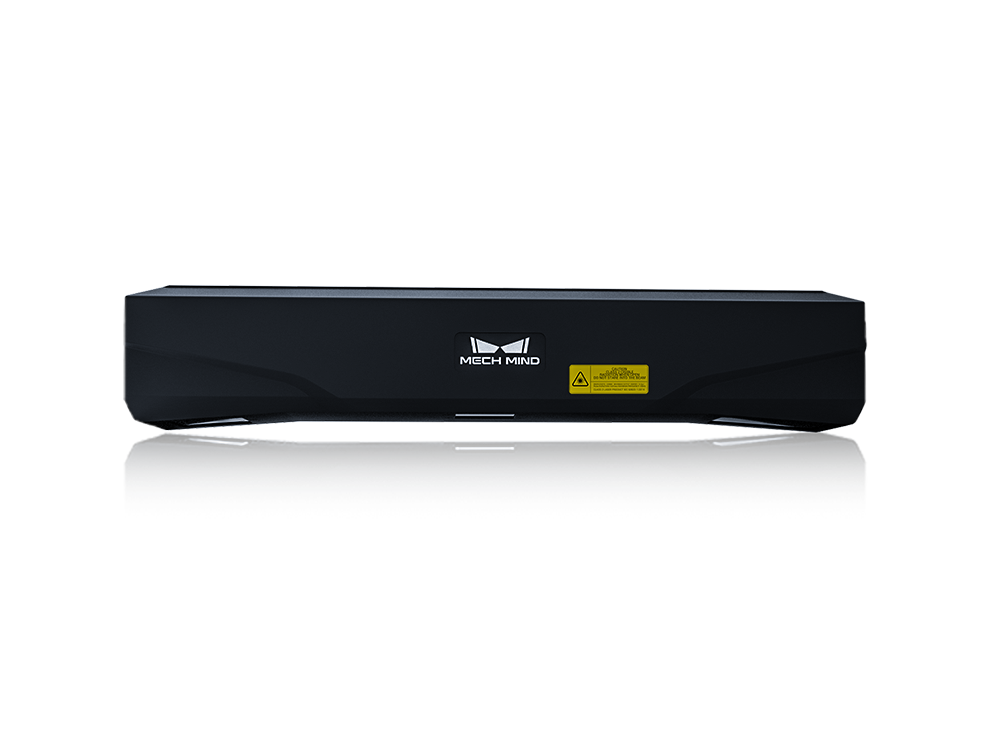
\includegraphics[width=\textwidth]{mechmind.png}
        \caption{Cámara 3D MechMind}
        \label{fig:mechmind}
    \end{minipage}
\end{figure}

\subsubsection{Garra Schunk}
Se utilizará una garra de la marca Schunk, compatible con el robot, para asegurar una sujeción fiable de las piezas. La selección de la garra se basará en el tamaño, forma y peso de las piezas a manipular.

\subsubsection{PLC Siemens 1200}
Controlador de reducido tamaño perfecto para la comunicación mediante protocolo Profinet.

\begin{figure}[h!]
    \centering
    \begin{minipage}{0.5\textwidth}
        \centering
        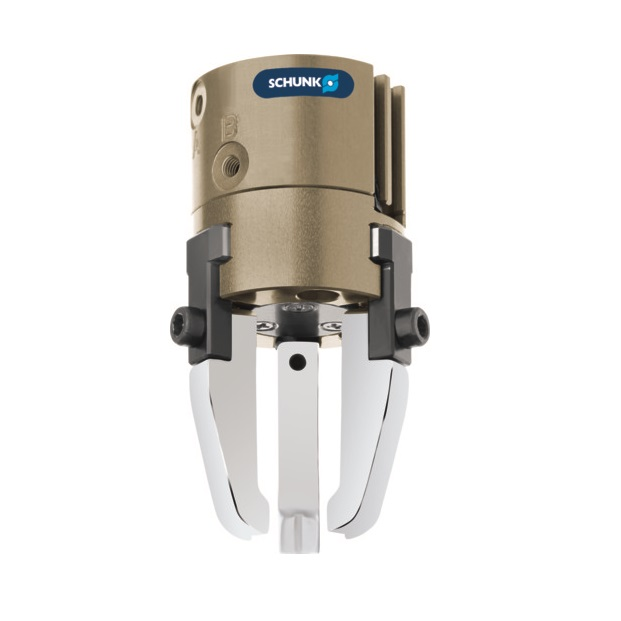
\includegraphics[width=\textwidth]{schunk.jpg}
        \caption{Garra Schunk.}
        \label{fig:schunk}
    \end{minipage}\hfill
    \begin{minipage}{0.4\textwidth}
        \centering
        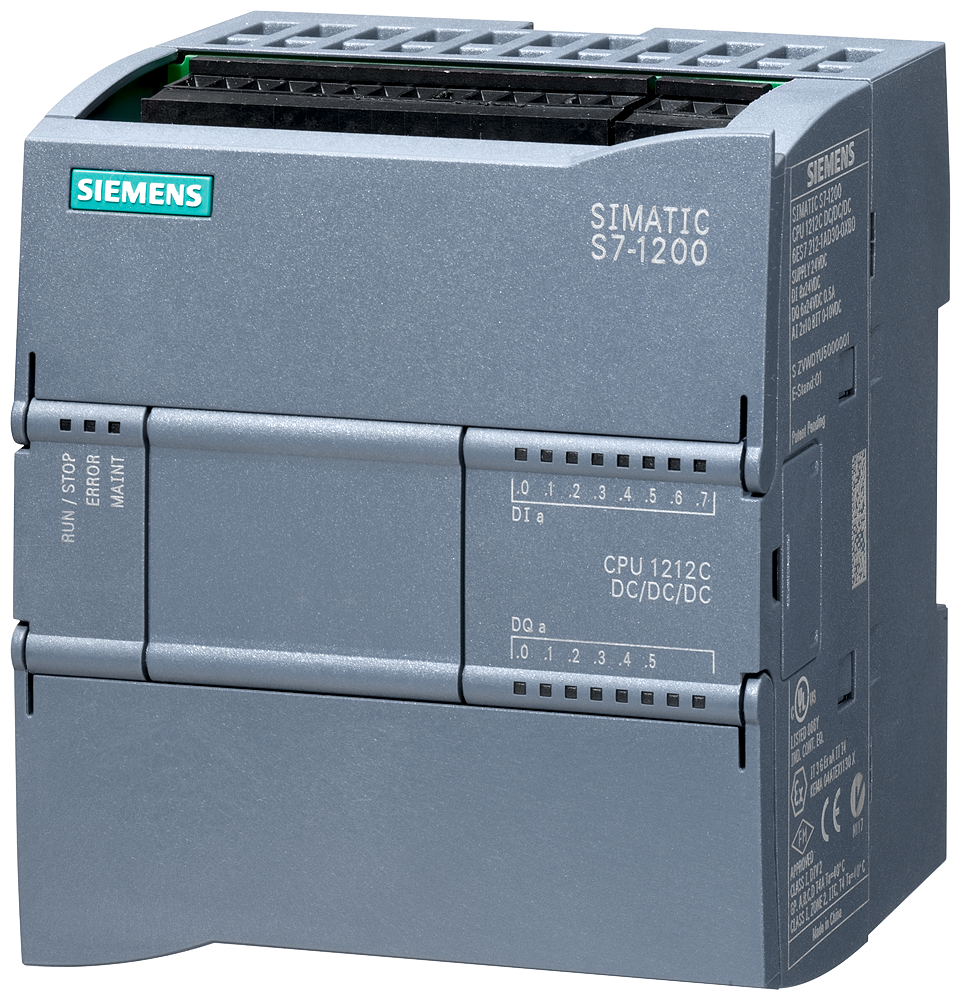
\includegraphics[width=\textwidth]{S1200.png}
        \caption{PLC Siemens S7-1200.}
        \label{fig:plc}
    \end{minipage}
\end{figure}

\subsubsection{Máquina de metrología Zeiss DuraMax}
La máquina Zeiss DuraMax será el componente principal para la inspección de calidad. Una vez que el robot presenta la pieza, el sistema de metrología ejecuta un programa predefinido para verificar sus dimensiones y tolerancias. El resultado de la inspección (pieza "buena" o "mala") se enviará al PLC, que determinará la siguiente acción del robot.

\begin{figure}[h!]
    \centering
    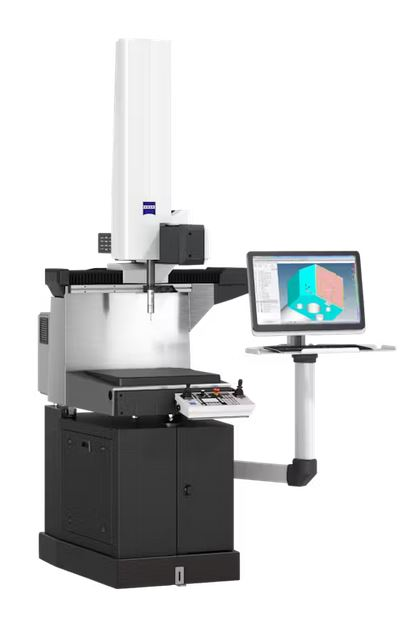
\includegraphics[width=0.5\textwidth]{duramax.JPG}
    \caption{Máquina de metrología Zeiss DuraMax.}
    \label{fig:duramax}
\end{figure}

\subsubsection{Software de tracking de producción}
Se desarrollará un software a medida para el seguimiento de la producción. Este sistema registrará y visualizará datos en tiempo real sobre el número de piezas procesadas, el tiempo de ciclo, los resultados de la inspección de calidad y el rendimiento general de la celda. Esto permitirá un análisis posterior y la optimización del sistema desde una perspectiva de gestión.

\section{Metodología}
La metodología del proyecto se ha definido para asegurar un desarrollo sistemático y eficiente, desde la planificación inicial hasta la validación final del sistema. El trabajo se ha estructurado en las siguientes fases:

\subsection{Diseño y planificación conceptual}
El punto de partida del proyecto es la conceptualización de la celda de manufactura.

\subsubsection{Diseño del layout de la celda}
Se definirá la disposición física de todos los componentes, como el robot, la máquina de metrología y el contenedor de piezas, optimizando el espacio de trabajo y minimizando las interferencias para una operación segura y eficiente.

\subsubsection{Selección de componentes}
Se seleccionará una garra Schunk y un sistema de visión 3D específicos, justificando su elección basándose en las características de las piezas a manipular y los requisitos de la aplicación de bin-picking.

\subsubsection{Definición de protocolos de comunicación}
Se establecerán los protocolos de comunicación entre el PLC Siemens y los demás dispositivos, asegurando un flujo de datos bidireccional y un control sincronizado de la celda.

\subsection{Simulación y validación virtual}
Se utilizará el software RoboDK para simular el proceso completo antes de la implementación física, lo que permitirá:

\subsubsection{Optimización de trayectorias}
Se programarán y optimizarán los movimientos del robot Dobot CR5 para reducir el tiempo de ciclo y mejorar la eficiencia en la manipulación de las piezas.

\subsubsection{Detección de colisiones}
Se validará el diseño de la celda en un entorno virtual para prevenir posibles colisiones entre el robot y otros componentes.

\subsection{Implementación y configuración del sistema}
Esta fase abarca la puesta en marcha de los diferentes subsistemas de la celda.

\subsubsection{Programación del robot Dobot CR5}
Se desarrollarán los programas de control para el robot, que gestionarán la secuencia del bin-picking y la transferencia de piezas a la máquina de metrología.

\subsubsection{Lógica de control en el PLC}
Se programará el PLC Siemens para gestionar la secuencia de trabajo, incluyendo las señales de inicio/fin de ciclo, los resultados de la metrología y la lógica de clasificación de piezas.

\subsubsection{Integración de componentes}
Se realizará la conexión física y la configuración de la red de comunicación entre todos los dispositivos de la celda.

\subsubsection{Desarrollo del software de tracking}
Se creará la aplicación que reciba datos del PLC para registrar y visualizar en tiempo real métricas de producción y calidad, como el número de piezas procesadas y el tiempo de ciclo.

\subsection{Pruebas y validación física}
Se llevarán a cabo pruebas exhaustivas para asegurar el correcto funcionamiento de toda la instalación.

\subsubsection{Pruebas de funcionamiento}
Se verificará que cada subsistema opere según lo planificado, desde la visión 3D hasta la respuesta de la máquina de metrología.

\subsubsection{Validación del proceso}
Se probará el sistema con piezas reales para asegurar la fiabilidad y precisión en la operación completa, desde la detección de piezas en el contenedor hasta su correcta clasificación.

\section{Resultados esperados}
Se espera que la finalización de este proyecto culmine con la consecución de los siguientes resultados tangibles y medibles:

\subsection{Implementación de la celda de manufactura}
La instalación completa de la celda de trabajo, con todos sus componentes (robot, máquina de metrología, garra, sistema de visión y PLC) integrados y operando de manera funcional y segura.

\subsection{Funcionamiento del sistema de bin-picking}
Un sistema de visión 3D plenamente operativo, capaz de detectar y localizar piezas de manera autónoma en un contenedor, y de comunicar sus coordenadas al robot para su correcta manipulación.

\subsection{Precisión en la metrología y clasificación}
La validación de que la máquina Zeiss DuraMax es capaz de realizar mediciones de alta precisión, y de que el PLC clasifica las piezas correctamente como "buenas" o "descartes" según los resultados de la inspección.

\subsection{Modelo de simulación validado}
La obtención de un modelo de simulación en RoboDK que represente fielmente el comportamiento de la celda física, lo que permitirá futuras optimizaciones y la demostración virtual del proceso.

\subsection{Software de tracking de producción}
Un sistema de software funcional que capture, almacene y visualice datos de producción en tiempo real, como el número de piezas procesadas, el tiempo de ciclo y los resultados de calidad.

\subsection{Documentación técnica completa}
La redacción de la memoria del TFG, un documento que no solo describa el proyecto y su metodología, sino que también actúe como un manual técnico para la operación de la celda y un informe de los resultados obtenidos.


\section{Planificación}
La planificación del proyecto se ha estructurado en fases para asegurar el cumplimiento de los objetivos dentro del plazo establecido. La siguiente tabla resume las actividades y su duración estimada.

\begin{center}
\begin{tabular}{|l|c|}
\hline
\textbf{Fase y Actividades} & \textbf{Duración (Semanas)} \\
\hline
\multicolumn{2}{|c|}{\textbf{Fase 1: Diseño y Planificación (Semanas 1-4)}} \\
\hline
Diseño de la celda y selección de componentes & 2 \\
Definición de protocolos de comunicación & 2 \\
\hline
\multicolumn{2}{|c|}{\textbf{Fase 2: Simulación y Programación (Semanas 5-10)}} \\
\hline
Simulación de la celda en RoboDK & 4 \\
Programación del PLC y del robot & 6 \\
\hline
\multicolumn{2}{|c|}{\textbf{Fase 3: Implementación y Pruebas (Semanas 11-16)}} \\
\hline
Integración de hardware y pruebas funcionales & 4 \\
Pruebas de validación del sistema & 2 \\
\hline
\multicolumn{2}{|c|}{\textbf{Fase 4: Documentación y Presentación (Semanas 17-20)}} \\
\hline
Redacción de la memoria del TFG & 4 \\
Preparación de la presentación final & 2 \\
\hline
\end{tabular}
\end{center}
\end{document}